\chapter{Получение признаков с использованием нейронных сетей}
\label{chapt2}

Описанный в главе \ref{chapt1} метод получения векторов признаков из столбцов
спектрограммы состоит из нескольких преобразований, каждое из которых опирается
на какие-то свойства музыкальных звукозаписей. Представление спектра звука в
виде вектора признаков необходимо, чтобы облегчить последующую классификацию.
Обучение представлениям -- это раздел машинного обучения, рассматривающий
алгоритмы, направленные на получение наилучших представлений входных данных.
Такие алгоритмы стремятся сохранить наиболее характерные признаки входных данных
в сжатом их представлении.

В основе многих алгоритмов обучения представлениям лежит многослойная нейронная
сеть. Важным свойством таких алгоритмов является возможность предварительного
обучения каждого слоя нейронной сети в отдельности без учителя, на неразмеченных
данных. Благодаря нему требуется существенно меньше размеченных данных для
окончательного обучения нейронной сети в целом.

В 2012 году Хамфри в \cite{Humphrey2012} предложил использовать один из методов
обучения представлениям -- свёрточные нейронные сети -- для получения признаков,
позволяющих классифицировать звучащий аккорд. В данной работе рассматривается
другой тип таких методов -- многослойные очищающие автоассоциаторы, в том числе
их рекуррентный вариант. Рекуррентные многослойные очищающие автоассоциаторы
были успешно использованы для распознавания речи в \cite{Maas2012}.

В разделе \ref{sect2_theory} даётся определение многослойного очищающего
автоассоциатора и сопутствующих понятий. В разделе \ref{sect2_sda} описывается
построение и обучение многослойной нейронной сети с использованием
автоассоциаторов, преобразующей столбец спектрограммы в вектор хроматических
признаков.

\section{Теоретические сведения и обзор литературы} \label{sect2_theory}

Определения в этом разделе даны в соответствии с \cite{Vincent2010}.

\emph{Автоассоциатор (автоэнкодер)} представляет из себя пару преобразований:
\begin{equation}
y = f_{\theta}(x) = s(Wx+b)
\end{equation}
\begin{equation} \label{g_theta}
z=g_{\theta'}(y) = s(W'y+b')
\end{equation}
Здесь $x$ -- входной вектор, $z$ -- реконструированный выходной вектор, $y$ --
\emph{внутреннее представление} для $x$, $\theta = \{W,b\}$ и
$\theta'=\{W',b'\}$ -- параметры (обычно накладывают ограничение $W'=W^T$), $s$
-- нелинейная функция активации (обычно это сигмоида или функция
гиперболического тангенса). Иногда в (\ref{g_theta}) выбирают в качестве $s$
линейную функцию. Автоассоциатор удобно представлять в виде нейронной сети с
одним скрытым слоем.

При обучении автоассоциатора минимизируется \emph{функция стоимости} $L(X,
Z(X)))$, где $X$ -- множество всех возможных входных векторов. Чтобы в процессе
обучения преобразования $f_{\theta}(x)$ и $g_{\theta}(y)$ не выродились в
тождественные, накладывают различные ограничения. Часто используемое
ограничение: размерность вектора $y$ должна быть меньше размерности входного
вектора $x$. Другой возможный вариант -- потребовать, чтобы размерность вектора
$y$ была больше размерности вектора $x$ и при этом большинство компонент $y$
были равны 0. При этом $y$ становится разреженным представлением вектора $x$.
Обозначим за $f_{\theta}^j(x)$ $j$-ю компоненту вектора $y$ при данном входном
векторе $x$. Тогда можем определить среднюю величину компонент вектора $y$:
\begin{equation}
\hat{\rho}_j = \frac{1}{m} \sum_{i=1}^m f_{\theta}^j(x^{(i)})
\end{equation}
Чтобы добиться $\hat{\rho}_j = \rho$, где $\rho$ -- параметр, контролирующий
разреженность, добавим слагаемое $L_{\rho}$ в функцию стоимости $L$. Это
слагаемое можно определять разными способами, в рамках данной работы будем
использовать следующую его форму, предложенную в \cite{NgCS294A}:
\begin{equation}
L_{\rho} = \beta \left[ \sum_{j=1}^h \left( \rho \log \frac{\rho}{\hat{\rho}_j} +
(1 - \rho) \log \frac{1 - \rho}{1 - \hat{\rho}_j} \right) \right]
\end{equation}
В дальнейшем будем использовать значение $\rho=0.05$, также в соответствии с
\cite{NgCS294A}.

\emph{Очищающий автоассоциатор} обучается таким образом, чтобы по повреждённому
(зашумлённому) вектору $\tilde{x}$ восстанавливать исходный вектор $x$.
Предполагается, что такие представления более устойчивы к помехам и лучше
отражают внутреннюю структуру входных данных. Показано \cite{Vincent2010}, что
во многих случаях внутренние представления, которые получаются при помощи
очищающего автоассоциатора, позволяют получить лучшие результаты в задачах
классификации по сравнению с представлениями, полученными при помощи обычных
автоассоциаторов. В \cite{Vincent2010} рассматриваются различные способы
получения зашумлённого вектора $\tilde{x}$.

Из автоассоциаторов можно строить многослойные модели, отождествляя нейроны из
скрытого слоя одного автоассоциатора со входными нейронами другого. В
полученной модели слои можно обучать друг за другом на неразмеченных данных.
Значения, полученные в скрытом слое последнего из автоассоциаторов, могут быть
использованы как векторы признаков.

РИСУНОК: многослойный автоассоциатор

Рекуррентный автоассоциатор может быть получен из обычного путём добавления
рекуррентных соединений, связывающих выходы скрытого слоя с дополнительными его
входами, по одному дополнительному входу на каждый выход. Фактически, при этом
получается сеть Эльмана, впервые описанная в \cite{Elman1990}. Промежуточное
представление $y(x_t)$ в таком случае вычисляется как
\begin{equation}
y(x_t) = s(Wx_t + b + Uy(x_{t-1}))
\end{equation}

РИСУНОК: рекуррентный многослойный автоассоциатор

\section{Построение нейронной сети и предобучение при помощи автоассоциаторов}
\label{sect2_sda}

Существенным недостатком многослойных автоассоциаторов является невозможность
содержательной интерпретации значений во внутреннем слое. В частности,
невозможно построить шаблонные наборы значений, соответствующие аккордам. Можно
попытаться обучить алгоритм классификации на векторах значений на выходах
внутреннего слоя. Но для случая 25 классов и достаточно большой размерности
векторов для обучения такого классификатора может потребоваться слишком много
данных.

Вместо этого соединим внутренный слой с дополнительным слоем, имеющим 12
выходов. Полученную нейронную сеть обучим на размеченных данных таким образом,
чтобы на выходе получались хроматические векторы (как в разделе
\ref{ssect1_chroma}), в которых каждая компонента соответствует одному
тональному классу. На вход этой сети будут подаваться столбцы спектрограммы.
Таким образом, вместо задачи классификации полученная нейронная сеть решает
задачу регрессии. Классификация же полученных 12-мерных векторов делается точно
так же, как и для других типов векторов признаков.

Предварительное обучение слоёв-автоассоциаторов будем производить методом
мини-пакетного (mini-batch) стохастического градиентного спуска (ССЫЛКА). При
этом сначала обучается первый слой на всём обучающем множестве, затем
полученные значения используются для обучения второго слоя, и так далее.
Окончательное обучение сети в целом также производится методом мини-пакетного
стохастического градиентного спуска.

Для очищающего автоассоциатора возможные помехи на входе можно смоделировать
при помощи аддитивного гауссового шума $\tilde{x}|x \sim \mathcal{N}(x,
\sigma_0^2 I)$, где $\sigma_0$ -- параметр. Это соответствует предположению о
том, что помехи равновероятны в любой области спектра. Возможны и другие
варианты моделирования помех. Для обучения последующих слоёв также будем
использовать эту модель шума с параметром $\sigma_i$ вместо $\sigma_0$ для
$i$-го слоя.

Естественным выбором для функции стоимости будет квадрат евклидова расстояния
между шаблоном и вектором на выходе (ССЫЛКА на другие варианты):
$$L(x,z) = ||x-z||^2$$
Для случая отсутствия аккорда в качестве соответствующего шаблона будем
использовать нулевой вектор.

В случае, когда в обучающей выборке большинство примеров соответствуют только
одному классу, очень вероятно получить в итоге сеть, которая все векторы будет
классифицировать как принадлежащие этому классу. В данном случае имеется 25
возможных классов, и желательно иметь приблизительно одинаковое количество
примеров на каждый класс. Однако не все аккорды используются в музыке одинаково
часто, и аккорд \emph{до-мажор} может встречаться в обучающей выборке в разы
чаще, чем \emph{фа-диез-мажор}.

Аналогичная проблема встречается и при обучении скрытых марковских моделей и
байесовских сетей для определения последовательности аккордов по
последовательности векторов признаков. В этих моделях часто используют
циклический сдвиг векторов признаков для усреднения параметров, соответствующих
разным аккордам. Этот процесс подробно описан, например, в \cite{Sheh2003}. Идея
его состоит в том, что, поскольку в хроматическом векторе каждая компонента
соответствует одному тональному классу, его циклический сдвиг даёт вектор,
соответствующий аккорду того же типа (мажорный или минорный) с основной нотой,
сдвинутой на полутон.

В данном случае при окончательном обучении нейронной сети в целом можно также
использовать сдвиг. Но входными векторами являются столбцы спектрограммы, и
циклический сдвиг соответствует неестественному переносу высокочастотных
компонент в область низких частот (или наоборот). Циклический сдвиг можно
эмулировать, добавив одну октаву к частотному диапазону спектрограммы, после
чего просто сдвигать по столбцу спектрограммы окно на октаву короче.

ЭКСПЕРИМЕНТ: а если делать просто циклический сдвиг?

При помощи такого сдвига из каждого столбца спектрограммы получается 12
различных столбцов, соответствующих 12 аккордам одного типа с разными основными
нотами. Это позволяет уравновесить количество аккордов в пределах одного типа.
Чтобы уравновесить количество аккордов между типами, потребуем, чтобы в процессе
генерации обучающей выборки из спектрограмм разница между общим количеством
мажорных аккордов и общим количеством минорных аккордов не превосходила
заданного числа $H$.

\section{Выводы}

\begin{enumerate}
  \item TODO
\end{enumerate}

%\newpage
%============================================================================================================================

\begin{figure} [h] 
  \center
  \includegraphics [scale=0.27] {LaTeX}
  \caption{TeX.} 
  \label{img:latex}  
\end{figure}

А это две картинки под общим номером и названием:
\begin{figure}[h]
  \begin{minipage}[h]{0.49\linewidth}
    \center{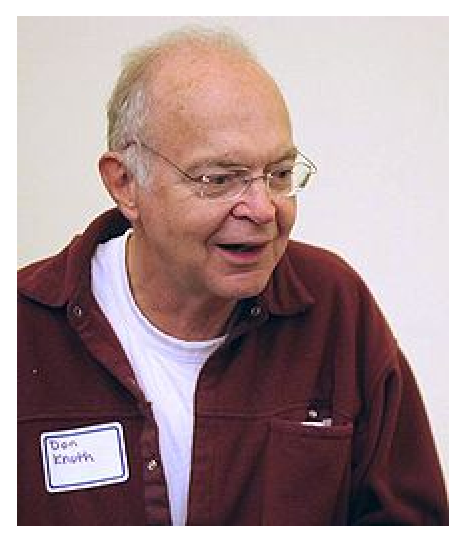
\includegraphics[width=0.5\linewidth]{knuth1} \\ а)}
  \end{minipage}
  \hfill
  \begin{minipage}[h]{0.49\linewidth}
    \center{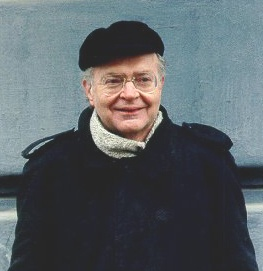
\includegraphics[width=0.5\linewidth]{knuth2} \\ б)}
  \end{minipage}
  \caption{Очень длинная подпись к изображению, на котором представлены две фотографии Дональда Кнута}
  \label{img:knuth}  
\end{figure}

%\newpage
%============================================================================================================================

\clearpage